% 
\documentclass[10pt]{article}
\usepackage{amscd,amsfonts,amssymb,amstext,latexsym} 
\usepackage{amsmath,mathbbol,mathrsfs,stmaryrd, mathtools} 
%\usepackage{mathbbol,mathrsfs,stmaryrd}
\usepackage {algorithm2e} 
\usepackage{theoremref}
\usepackage[T1]{fontenc}
\usepackage[english]{babel} 
\usepackage {enumerate}
\usepackage{url}
%\usepackage {algpseudocode}  
\usepackage{graphics} 
\usepackage{tikz}
%\usepackage[square]{natbib}
\usepackage[width=14.8cm,left=3cm]{geometry}
\usetikzlibrary{automata,calc}
%\usepackage{tgtermes} 
\usepackage{listings}
\usepackage{mathptmx}
\usepackage{fancyhdr}
\usepackage{verbatim}
\usepackage{float}
\usepackage{enumitem}
\usepackage{booktabs}
\usepackage[flushleft]{threeparttable}
\usepackage{listings}
\usepackage{verbatim}
\usepackage{fancyhdr}
\usepackage{multirow,multicol}
\usepackage[colorlinks=true,linkcolor=blue,citecolor=blue,urlcolor=blue]{hyperref}
\usepackage{tabto}
\lstset{ %
language=C++,                % choose the language of the code
basicstyle={\ttfamily},       % the size of the fonts that are used for the code
backgroundcolor=\color{white},  % choose the background color. You must add \usepackage{color}
showspaces=false,               % show spaces adding particular underscores
aboveskip=6mm, 
%belowskip=3mm, 
numbers=left, numberfirstline=false, numberblanklines=false,
numberstyle=\tiny\color{gray}, numbersep= 5pt, 
showstringspaces=false,         % underline spaces within strings
showtabs=false,                 % show tabs within strings adding particular underscores
%frame=single,           % adds a frame around the code
%frame = tb, 
frame = none, 
tabsize=2,          % sets default tabsize to 2 spaces
captionpos=b,           % sets the caption-position to bottom
breaklines=true,        % sets automatic line breaking
breakatwhitespace=false,    % sets if automatic breaks should only happen at whitespace
escapeinside={\%*}{*)}          % if you want to add a comment within your code
}
%\graphicspath{{../../pics/}}
\fancypagestyle{plain}{
\fancyhf{}
\rhead{School of Computer Science and Applied Mathematics\\ 
%\noindent\rule{15.4cm}{0.4pt}\\
\footnotesize{\textsc{University of the Witwatersrand, Johannesburg}}}
\lhead{
\includegraphics[scale=0.08]{witslogo_h.png}}
\fancyfoot[C]{\thepage}
\renewcommand{\headrulewidth}{0.4pt}
}

\textwidth=16.8cm 
\textheight=22.6cm 
\evensidemargin 0pt 
\oddsidemargin 0pt 
\leftmargin 0pt 
\rightmargin 0pt 
\setlength{\topmargin}{0pt} 
\setlength{\footskip}{50pt}
\setlength{\parindent}{0pt}
\setlength{\parskip}{1em}
\linespread{1} 
% 
\makeatletter
\newcommand{\rmnum}[1]{\romannumeral #1}
\newcommand{\Rmnum}[1]{\expandafter\@slowromancap\romannumeral #1@}
\makeatother

\begin{document}
\title{COMS4036A Project - Gaussian Mixture Models}
\author{Angus Mackenzie - 1106817}
\date{\today} 
\maketitle 
%\thispagestyle{empty}
\pagestyle{fancy}
\fancyhf{}
\fancyhead[R]{\thepage}
\fancyhead[L]{COMS4036A}
%\vskip 3mm 
%\pagenumbering{roman}
%\newpage
\pagenumbering{arabic}
\section{Introduction}
In this project we were tasked with building a Gaussian Mixture Model (GMM) \cite{princeCVMLI2012} that can detect coins in an image. The aim was to produce a mask that would show coin pixels in white and desk pixels in black.

\section{Experimental Methodology}
\subsection{Data Exploration}
Initially a portion of the data was loaded and some cursory exploration done. Then the remaining images were loaded, normalised, and flattened. Finally, they were split into a training set and test set, with 80\% of the images set aside for training. 

\subsection{Algorithms}
The fundamental algorithm of a GMM is Expectation Maximisation \cite{princeCVMLI2012}, which consist of two steps, the Expectation step (E-step) and the Maximisation step (M-step). 

The E-step is where we find the posterior probability distribution of the hidden variable. This is represented as:
$$
\begin{aligned} q_{i}\left(h_{i}\right)=\operatorname{Pr}\left(h_{i}=k | \mathbf{x}_{i}, \boldsymbol{\theta}^{[t]}\right) &=\frac{\operatorname{Pr}\left(\mathbf{x}_{i} | h_{i}=k, \boldsymbol{\theta}^{[t]}\right) \operatorname{Pr}\left(h_{i}=k, \boldsymbol{\theta}^{[t]}\right)}{\sum_{j=1}^{K} \operatorname{Pr}\left(\mathbf{x}_{i} | h_{i}=j, \boldsymbol{\theta}^{[t]}\right) \operatorname{Pr}\left(h_{i}=j, \boldsymbol{\theta}^{[t]}\right)} \\ &=\frac{\lambda_{k} \operatorname{Norm}_{\mathbf{x}_{i}}\left[\boldsymbol{\mu}_{k}, \Sigma_{k}\right]}{\sum_{j=1}^{K} \lambda_{j} \operatorname{Norm}_{\mathbf{x}_{i}}\left[\boldsymbol{\mu}_{j}, \Sigma_{j}\right]} \\ &=r_{i k} \end{aligned}
$$ \cite{princeCVMLI2012}.

The M-step maximises our parameters, this can be represented as:
$$
\begin{aligned} \lambda_{k}^{[t+1]} &=\frac{\sum_{i=1}^{I} r_{i k}}{\sum_{j=1}^{K} \sum_{i=1}^{I} r_{i j}} \\ \boldsymbol{\mu}_{k}^{[t+1]} &=\frac{\sum_{i=1}^{I} r_{i k} \mathbf{x}_{i}}{\sum_{i=1}^{I} r_{i k}} \\ \Sigma_{k}^{[t+1]} &=\frac{\sum_{i=1}^{I} r_{i k}\left(\mathbf{x}_{i}-\boldsymbol{\mu}_{k}^{[t+1]}\right)\left(\mathbf{x}_{i}-\boldsymbol{\mu}_{k}^{[t+1]}\right)^{T}}{\sum_{i=1}^{I} r_{i k}} \end{aligned}
$$
\cite{princeCVMLI2012}

Initially, the two methods for both the E and M steps were completed in order to test the accuracy of their output on dummy data.

\subsection{Testing}
 Training images were run through the EM algorithm with the number of components set to 2 in order to ascertain whether the system was functional. After that models with components of value 1-10 were trained, and their accuracy over all the test data averaged. 

\section{Results \& Analysis}
In the data exploration phase of the methodology, the main goal was to ascertain what colour space would be most beneficial for the GMM. A plot containing the different  colour components was created:

\begin{figure}[H]
    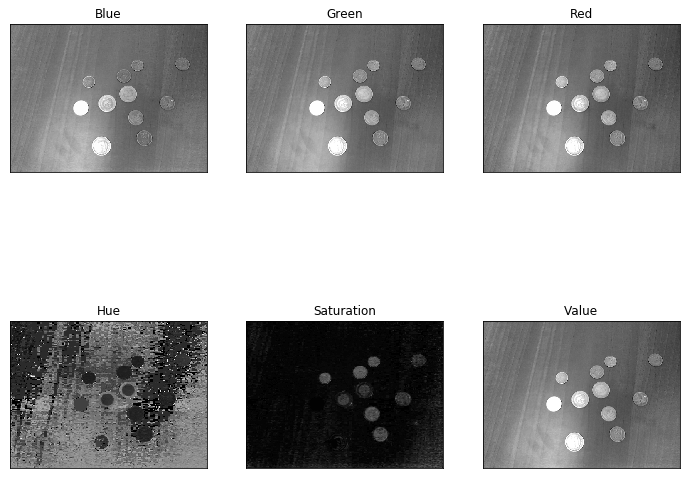
\includegraphics[width=0.7\textwidth]{Components}
    \centering
\end{figure}

From this plot it can be seen that the different components add different information. I decided to use the Value component from the HSV colour space as colour information in the RGB colour space can be more noisy than HSV information. 

The E-step was tested using data from the 2017 Master's students Exam memo \cite{exam}, it achieved the correct results. The same can be said of the M-step, using the 2017 Test 2 paper memo \cite{test}.

The first stage of testing was simply to verify that the GMM could produce meaningful outputs. This was achieved, with some results better than others:
\begin{figure}[H]
    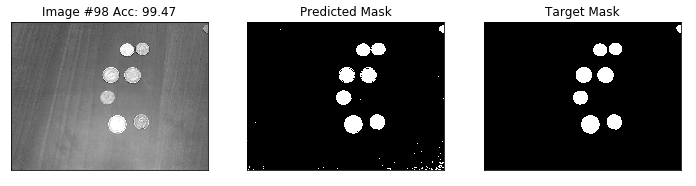
\includegraphics[width=\textwidth]{98}
    \centering
\end{figure}

In the above image we can see that the mask created from the image is very close to the target. There are slight bits of noise that reduce the accuracy marginally, but that can be remedied through the use of digital image processing techniques like filtering.

\begin{figure}[H]
    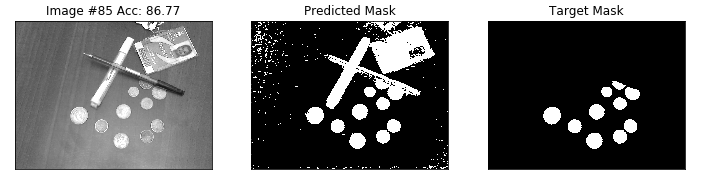
\includegraphics[width=\textwidth]{85}
    \centering
\end{figure}

The above mask has a lower accuracy, as the items in the photo have been misclassified by the GMM as coins, and thus made white.

Through testing it is apparent that the amount of components does little to increase the accuracy of the GMM in any meaningful way, and only increases the time taken to process new data. 

\begin{figure}[H]
    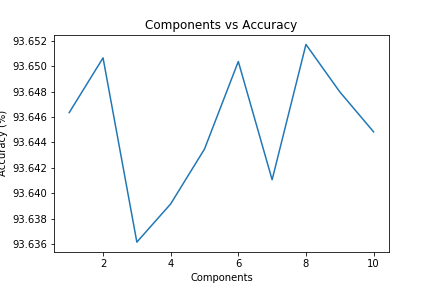
\includegraphics[width=0.7\textwidth]{acuracyc}
    \centering
\end{figure}

The above graph shows the number of components used by the GMM vs the accuracy, and the changes in accuracy are miniscule for the added components. 

\begin{figure}[H]
    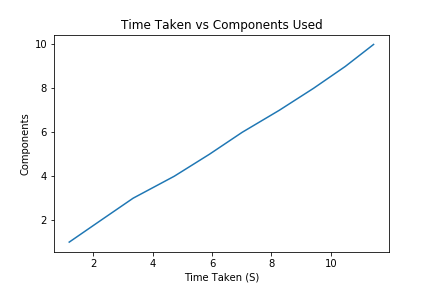
\includegraphics[width=0.7\textwidth]{Timetaken}
    \centering
\end{figure}


There is a strong direct relation between the number of components used by the GMM and the time elapsed during the testing phase.

\section{Conclusion}
Thus, it can be seen that a GMM can work surprisingly well as a means of masking and image segmentation for basic tasks.

\bibliographystyle{plain}
\bibliography{references}
\end{document} 
